\chapter{Curvatura geodésica y geodésicas}

\section{Curvatura geodésica}
\large 

El vector de curvatura $\mathbf{k}$ de una curva $C$ en una superficie $S$ puede descomponerse en dos componentes, como hemos visto en el capítulo anterior. Una de estas componentes es paralela a $\mathbf{n}$ y se conoce como \emph{curvatura normal}. La otra componente se denomina \emph{curvatura geodésica}. 
\begin{wrapfigure}{r}{.4\textwidth}
    \centering
    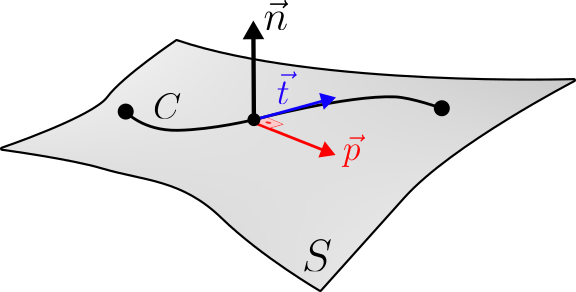
\includegraphics[scale=.4]{FOTOS/curva_geo_1.png}
    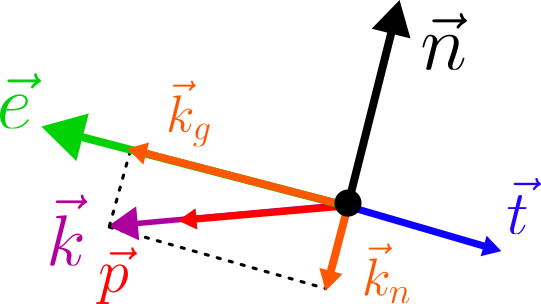
\includegraphics[scale=.4]{FOTOS/curva_geo_2.png}
\end{wrapfigure}
$$
\mathbf{k}=\mathbf{k}_n+\mathbf{k}_g
$$
donde $\mathbf{k}=k\mathbf{p}$. Si nos fijamos en el plano formado por $\mathbf{k}$ y $\mathbf{k}_n$, como $\mathbf{n}\perp \mathbf{t}\perp \mathbf{p}$, $\mathbf{k}_g\propto \mathbf{e}$, donde $\mathbf{e}=\mathbf{n}\wedge \mathbf{t}$; luego lo que ocurre es que $k_g=\mathbf{e\cdot k}=(\mathbf{n}\wedge \mathbf{t})\cdot \mathbf{k}$.\\

Si ahora usamos las fórmulas de Frenet, en parametrización natural,
\begin{gather*}
    \mathbf{k}=\Ddot{\mathbf{x}} \quad , \quad \mathbf{t}=\dot{\mathbf{x}} \quad , \quad ||\dot{\mathbf{x}}||=1 \ \forall \ s\\
    k_g=(\mathbf{n}\wedge \dot{\mathbf{x}})\cdot \ddot{\mathbf{x}}=[\ddot{\mathbf{x}}\ ,\ \dot{\mathbf{x}}\ ,\ \mathbf{n}]\\
    \boxed{k_g=\det{\mathbf{n}\ | \ \dot{\mathbf{x}}\  | \ \ddot{\mathbf{x}}}}
\end{gather*}
En parametrización arbitraria:
$$
\dv{}{S}=\dv{t}{S}\cdot \dv{}{t}=\frac{1}{||\mathbf{x}'||}\dv{}{t}
$$
luego:
\begin{gather*}
    \dot{\mathbf{x}}=\frac{\mathbf{x}'}{||\mathbf{x}'||}\longrightarrow \ddot{\mathbf{x}}=\frac{\mathbf{x}''}{||\mathbf{x}'||^2}+\frac{1}{||\mathbf{x}'||}\cancelto{\text{\parbox{2.55cm}{\small No contribuye al determinante}}}{\left ( \dv{}{t} \left ( \frac{1}{||\mathbf{x}'||} \right ) \right )}\cdot \mathbf{x}'\\
    \boxed{k_g=\frac{1}{||\mathbf{x}'||^3}\det{\mathbf{n} \ | \ \mathbf{x}' \ | \ \mathbf{x}''}}
\end{gather*}
\section{Geodésicas}
Una \emph{pregeodésica} es una es una curva con \emph{curvatura geodésica nula} en cualquier punto de la curva.\\

Una \emph{geodésica} es una curva que:
\begin{enumerate}
    \item Es \emph{pregeodésica}, $k_g=0$
    \item Tiene un vector velocidad \emph{constante}, $||\mathbf{x}'||\equiv $ const.
\end{enumerate}

Si reparametrizamos una geodésica, $k_g$ seguirá siendo nulo, pero puede que la velocidad deje de ser constante. En consecuencia, una curva pregeodésica siempre mantiene su condición de pregeodésica.\\

Por otro lado, una geodésica es una pregeodésica parametrizada en su parámetro afín, donde el parámetro afín es una transformación lineal de la longitud de arco.
$$
t_\text{afín}=aS+b\ , \qquad a,b\equiv \text{const.} 
$$
\begin{mybox}
    \underline{Ejemplo A:} $\mathbf{x}(t)=(\log t,\log t,\log t)$ es una pregeodésica
    $$
    k_g=\frac{1}{||\mathbf{x}'||}\det{\mathbf{n} \ | \ \mathbf{x}' \ | \ \mathbf{x}''}=0 \ , \ ||\mathbf{x}'||\not \equiv \text{const.}
    $$
    $
    \mathbf{x}(\Bar{t})=(\Bar{t},\Bar{t},\Bar{t}) \ (\Bar{t}=\log t)\ \iff \mathbf{x}(t)
    $ cumple que $k_g=0$ y  $||\mathbf{x}'||\equiv \text{const.}  \ \forall \ \Bar{t}$. Es decir, $\mathbf{x}(\Bar{t})$ es una geodésica.
\end{mybox}

Un resultado muy importante es que la condición de $||\mathbf{x}'||\equiv $ const. de las geodésicas implica que, en una geodésica, la aceleración es \emph{paralela a} $\mathbf{n}$. El razonamiento es el siguiente:
\begin{align*}
    \dv{}{t}||\mathbf{x}'||^2=\mathbf{0}&\implies (\mathbf{x}'\cdot \mathbf{x}')'=\mathbf{x}''\cdot \mathbf{x}' +\mathbf{x}'\cdot \mathbf{x}''=2\mathbf{x}'\cdot \mathbf{x}''=\mathbf{0}\\
    &\iff \mathbf{x}'\perp \mathbf{x}''
\end{align*}
Además, $k_g=0=(\mathbf{n}\wedge \mathbf{x}')\cdot \mathbf{x}''$. Esto significa que $\mathbf{n,x',x''}$ son coplanares, lo que implica que $\mathbf{n}\parallel \mathbf{x}''$.\\

Las consecuencias de este resultado son que las rectas (con curvatura nula) son siempre pregeodésicas en cualquier superficie que las contiene.
\begin{mybox}
    \underline{Ejemplo B:} $S$: Paraboloide hiperbólico: $\mathbf{x}(u,v)=(u,v,u^2-v^2)$.\\
    La curva $\mathbf{x}(t)=(t,t,0)$ es una recta, y por tanto una pregeodésica (además de geodésica)
\end{mybox}
\newpage
    \begin{figure}[!h]
        \centering
        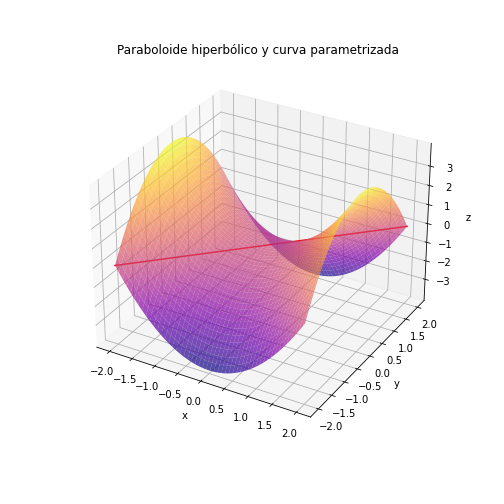
\includegraphics[scale=.5]{FOTOS/hiperb_curva.png}
        \caption*{Ejemplo B: Paraboloide hiperbólico y geodésica}
        \label{fig:ej4B}
    \end{figure}
\begin{wrapfigure}{r}{0.2\textwidth}
    \centering
    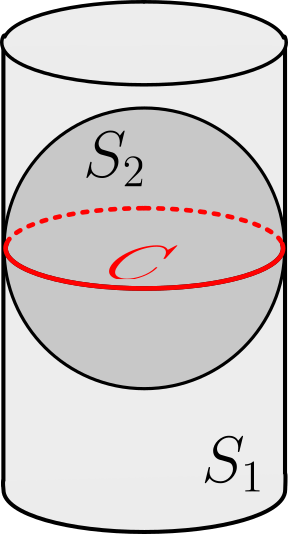
\includegraphics[scale=.35]{FOTOS/cilindro_geo.png}
\end{wrapfigure}

Si $S_1$ y $S_2$ son dos superficies tangentes entre sí a lo largo de una cierta curva $C$, entonces el hecho de que $C$ sea pregeodésica de $S_1$ implica que también lo es de $S_2$.
\subsection{Ecuación de las geodésicas}
Sea $C$ una curva sobre una superficie $S$:
$$
\mathbf{x}(s)=\mathbf{x}(u^1(s),u^2(s))=\mathbf{x}(u^\alpha (s))
$$
\begin{equation*}
    \begin{split}
        \mathbf{k}=k\mathbf{p} =\ddot{\mathbf{x}} \quad , \quad \mathbf{k}&=\mathbf{k}_g+\mathbf{k}_n\\
        &=\mathbf{k}_g+k\cdot \mathbf{n}
    \end{split}
\end{equation*}
$\mathbf{k}_g$ es la parte de $\ddot{\mathbf{x}}$ que es perpendicular a $\mathbf{n}$. 
\begin{equation*}
    \begin{split}
        \dot{\mathbf{x}}=\mathbf{x}_\alpha \cdot \dot{u}^\alpha \implies \ddot{\mathbf{x}}&=\mathbf{x}_{\alpha \beta }\cdot \dot{u}^\alpha \dot{u}^\beta +\mathbf{x}_\alpha \cdot \ddot{u}^\alpha \\
        \ref{gauss} \rightarrow &=(\Gamma _{\alpha \beta }{}^\gamma \cdot \mathbf{x}_\gamma +b_{\alpha \beta }\cdot \mathbf{n})\dot{u}^\alpha \dot{u}^\beta +\mathbf{x}_\alpha \cdot \ddot{u}^\alpha \\
        &=\underbrace{(\ddot{u}^\gamma +\Gamma _{\alpha \beta }{}^\gamma \dot{u}^\alpha \dot{u}^\beta )}_{\mathbf{k}_g}\ \mathbf{x}_\gamma + \underbrace{b_{\alpha \beta }\dot{u}^\alpha \dot{u}^\beta }_{\mathbf{k}_n}\ \mathbf{n}
    \end{split}
\end{equation*}
\WFclear
La condición de geodésica, $k_g=0$, además de que la velocidad sea constante, implica que, para este tipo de curva, se cumple la siguiente ecuación diferencial
$$
\ddot{u}^\gamma +\Gamma _{\alpha \beta }{}^\gamma \dot{u}^\alpha \dot{u}^\beta=0
$$
donde los símbolos de Christoffel se evalúan sobre la curva. Si escribimos las derivadas explícitamente, entonces:
$$
\boxed{\dv[2]{u^\gamma }{s}+\Gamma _{\alpha \beta }{}^\gamma \dv{u^\alpha }{s}\dv{u^\beta }{s}=0} \qquad \qquad \left ( \text{\small \parbox{5cm}{\begin{center}
    La estructura de esta ecuación es válida para parámetros afines $t_a=aS+b$. Al resolver esta ecuación, se obtienen las curvas en parámetro afín.
\end{center}}} \right )
$$
La ecuación es válida si trabajamos en una variedad de dimensión $n$ (en Relatividad General, se usará como parámetro $s$ el tiempo propio, $\lambda $).
\begin{mybox}
    \underline{Ejemplo C:} Plano $XY$ en coordenadas cartesianas.
    $$
    \mathbf{x}(u^1,u^2)=(u^1,u^2,0) \longrightarrow g_{\alpha \beta }=\mathbb{1}_{2\times 2} \ , \ \Gamma _{\alpha \beta }{}^\gamma =0
    $$
    Las geodésicas cumplirán:
    $$
    \dv[2]{u^\gamma }{s}=0\implies \left \{ \begin{array}{ccc}
         \dv[2]{u^1}{s}=0&\implies&u^1=as+b   \\\\
         \dv[2]{u^2}{s}=0&\implies&u^2=cs+d 
    \end{array} \right \} \ a,b,c,d \in \mathbb{R}
    $$
\end{mybox}
\section{Propiedades extremales de las geodésicas: arcos de longitud mínima}
\begin{wrapfigure}{l}{0.35\textwidth}
    \centering
    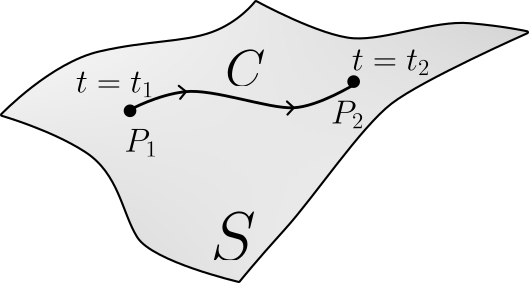
\includegraphics[scale=.4]{FOTOS/min_arco1.png}
    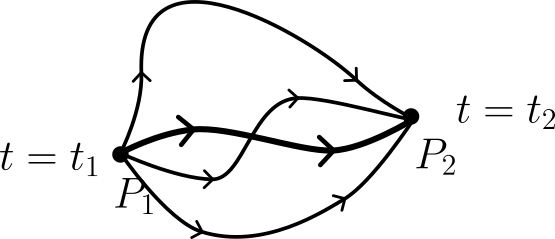
\includegraphics[scale=.35]{FOTOS/min_arco2.png}
\end{wrapfigure}
La longitud de arco de la curva $C$ contenida en la superficie $S$ que va desde el punto $P_1$ hasta el punto $P_2$ es:
$$
\ell =\int _{t_1}^{t_2} \odif{t} \sqrt{g_{\alpha \beta }(u^\alpha )'(u^\beta )'} \quad g_{\alpha \beta }=\mathbf{x}_\alpha \cdot \mathbf{x}_\beta 
$$
El integrando en la longitud de arco puede entenderse como un lagrangiano en Mecánica Clásica, que depende de las coordenadas $(u^1,u^2)$ y sus velocidades $((u^1)',(u^2)')$:
$$
\mathcal{L}(u^\alpha ,(u^\beta )')=\sqrt{g_{\alpha \beta }(u^\alpha )'(u^\beta )'}
$$
Y si pedimos que el arco que une $P_1$ y $P_2$ sea de longitud mínima, tenemos que imponer que se cumplan las \emph{ecuaciones de Euler-Lagrange} (es decir, usamos un método variacional):
$$
\boxed{\pdv{\mathcal{L}}{u^\mu }-\dv{}{t}\pdv{\mathcal{L}}{(u^\mu )'}=0}
$$
$$\hookrightarrow \pdv{\mathcal{L}}{u^\mu }=\frac{1}{2\sqrt{g_{\alpha \beta }(u^\alpha )'(u^\beta )'}}\pdv{g_{\alpha \beta }}{u^\mu }\cdot (u^\alpha )'(u^\beta )' $$
\begin{equation*}
    \begin{split}
        \hookrightarrow \pdv{\mathcal{L}}{(u^\mu )'}&=\frac{1}{2\sqrt{g_{\alpha \beta }(u^\alpha )'(u^\beta )'}}\left [ g_{\rho \sigma } \underbrace{\pdv{(u^\rho )'}{(u^\mu )'}}_{\delta ^\rho {}_\mu }\cdot (u^\sigma )'+g_{\rho \sigma }(u^\rho )'\underbrace{\pdv{(u^\sigma )'}{(u^\mu )'}}_{\delta ^\sigma {}_\rho } \right ]\\
        &=\frac{1}{\sqrt{g_{\alpha \beta }(u^\alpha )'(u^\beta )'}} g_{\mu \sigma }(u^\sigma )'
    \end{split}
\end{equation*}
Este resultado es general hasta este punto y no depende de la parametrización de $C$. A partir de ahora, realizaremos el resto del cálculo \emph{en parametrización natural}.
\begin{align*}
    \pdv{\mathcal{L}}{\dot{u}^\mu }&= g_{\mu \sigma } \dot{u}^\sigma \\
    \pdv{\mathcal{L}}{u^\mu }&=\frac{1}{2}\pdv{g_{\rho \sigma }}{u^\mu }\dot{u}^\rho \dot{u}^\sigma \\
    \dv{}{s}\left ( \pdv{\mathcal{L}}{\dot{u}^\mu } \right )&=\dot{g}_{\mu \sigma }\dot{u} ^\sigma +g_{\mu \sigma }\ddot{u}^\sigma \\
    &=\pdv{g_{\mu \sigma }}{u^\rho }\cdot \dot{u}^\rho \dot{u}^\sigma +g_{\mu \sigma }\ddot{u}^\sigma 
\end{align*}
\begin{gather*}
    g_{\mu \sigma }\ddot{u}^\sigma +\pdv{g_{\mu \sigma }}{u^\rho }-\frac{1}{2} \pdv{g_{\rho \sigma }}{u^\mu }\dot{u}^\rho \dot{u}^\sigma=0\\
    \ddot{u}^\nu +\frac{1}{2}g^{\nu \mu }\left ( \pdv{g_{\mu \sigma }}{u^\rho }+\pdv{g_{\mu \rho }}{u^\sigma }-\frac{1}{2}\pdv{g_{\rho \sigma }}{u^\mu } \right )\dot{u}^\rho \dot{u}^\sigma =0\\
    \implies \boxed{\ddot{u}^\nu +\Gamma _{\rho \sigma }{}^\nu \dot{u}^\rho \dot{u}^\sigma=0} \qquad \text{ Ecuación de las geodésicas}
\end{gather*}
Es decir, las geodésicas son arcos de longitud mínima en la superficie parametrizada S.


